\documentclass{article}
\usepackage[utf8]{inputenc}
\usepackage{times}
\usepackage{latexsym}
\usepackage{acl2020}
\usepackage{graphicx}

\title{Working Title}

\author{
James Blackburn (jimbb82@uw.edu)\\
Joshua Valdez (jdv2@uw.edu)\\
Joseph Nollette (nollejos@uw.edu)\\
Christian Kavouras (cdkavour@uw.edu)
}

\date{\vspace{-5ex}}

\begin{document}

\maketitle

\begin{abstract}
We present a system for predicting the humor content of English-language news article headlines; specifically, the boost in perceived humor resulting from the replacement of one word or phrase in the original headline with a new word, as rated by human judges.
\end{abstract}

\section{Introduction}
SemEval-2020 Task 7 seeks to expand upon the task of predicting the humor content of chunks of text, and attempts to measure the change in human-judged humor values when individual words are replaced. We will build a system that -- given original chunks and edited chunks -- will predict the mean humor score of an edited headline.

\section{Task Description}
The primary task of this project is to implement a regression model to predict the degree of humor of brief news headlines, using data from the Humicroedit data set. This data set contains the text of news headlines in which one word has been edited to change a serious headline into a humorous one. All training instances contain the full text of the headline, the word that was replaced, the new word that was put in its place, and a decimal score between 0 (not funny) and 3 (very funny), obtained by taking the average score given by five human judges. The description of this task and its dataset can be found \href{https://competitions.codalab.org/competitions/20970}{here}.\cite{hossain-etal-2019-president}

The adaptation task we plan to complete is to apply a similar model, trained on both the original and edited headlines referenced above, to tweets. The goal is to predict the humor content of tweets according to the same scale and, by employing a time-series clustering algorithm, explore the correlation of the frequency of humorous posts on social media to certain periods of time.

\section{System Overview}

We have chosen to interpret the primary task as a regression problem, using a bidirectional encoder representation from transformers (BERT) model to predict the humor content of edited headlines.

This model \cite{DBLP:journals/corr/abs-1810-04805} consists essentially of a series of transformer encoders which takes embeddings of labeled headlines as its input and generates a predictied humor score for each instance. The task will be completed by generating pretrained models and then proceeding to a fine-tuning phase to improve performance.

% \vspace{1cm}
\begin{figure}
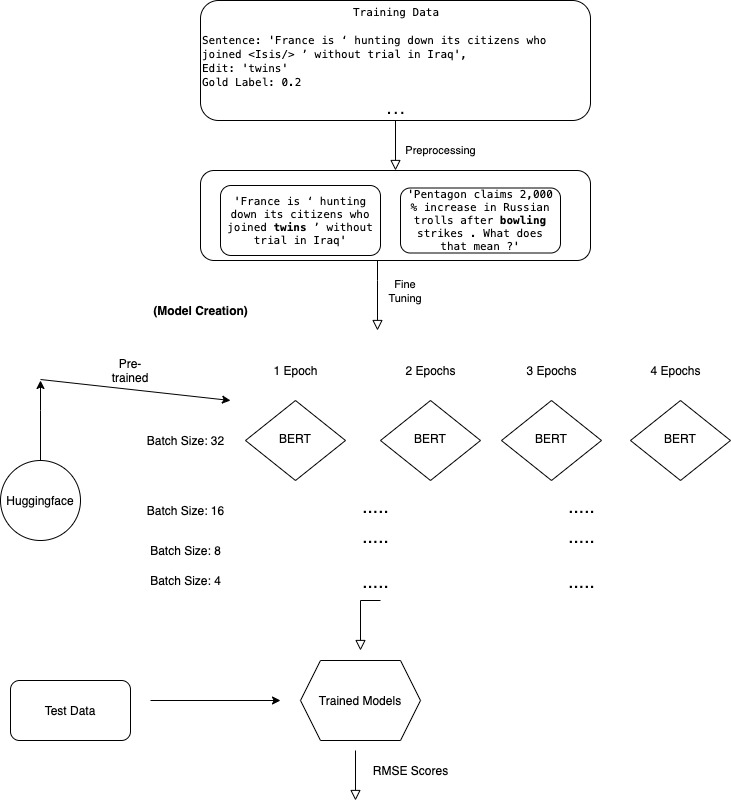
\includegraphics[scale=0.25]{classifier.jpg}
\caption{System Architecture for our primary task prediction}
\end{figure}
% \vspace{1cm}

To complete the pretraining phase, sixteen distinct models were generated from embeddings of the labeled training instances, by varying the number of training epochs from one to four, and employing batch sizes of 4, 8, 16, and 32 instances. A root mean square error is employed as the loss function.

\section{Results}

Below is a table of the RMSE values for the sixteen combinations of epochs and batch size. Our Baseline value was formulated using the RMSE across the label values of our training and test data.

results for subtask1:
baseline: 0.57471
BERT single regressor:
task A RMSE results:
\begin{center}
\begin{tabular}{|c|c|c|c|c|}
\hline
epochs & batch=32 & batch=16 & batch=8 & batch=4 \\
\hline
1epochs & 0.54199 & 0.54312 & 0.53396 & 0.53438 \\
2epochs & 0.53324 & 0.54381 & 0.5383 & 0.54047 \\
3epochs & 0.54728 & 0.54737 & 0.56014 & 0.55393 \\
4epochs & 0.55964 & 0.55747 & 0.56742 & 0.56569 \\
\hline
\end{tabular}
\end{center}

As shown, the best result we have obtained from this initial run is from 2 epochs and a batch size of 32.

\section{Discussion}

From this initial phase, we aim to explore methods for fine-tuning BERT, as well as the potential of expanding our approach from single regression to multiple regression. In a similar task using a multi-lingual data set, the highest performing model makes use of a Gradient Boosted Layer on top of BERT \cite{Ismailov2019HumorAB}. This could be a place of further exploration for improving performance.

\section{Conclusion}

\bibliographystyle{acl_natbib}
\bibliography{refs}

\end{document}
